\documentclass[12pt,a4paper]{report}
\usepackage{graphicx}
\usepackage{fancyhdr}
\usepackage{lastpage}
\usepackage{titlesec}
\usepackage{tabularx}
\usepackage{xcolor,colortbl}
\usepackage{multirow}
\usepackage[sfdefault]{roboto}
\usepackage[T1]{fontenc}
\usepackage{subfig}
\usepackage{wrapfig,lipsum,booktabs}

\usepackage{geometry}
% \geometry{
%  a4paper,
%  left=35mm,
%  top=35mm,
%  }


\setlength{\parindent}{0pt}
\bibliographystyle{plain}


\definecolor{LightCyan}{rgb}{0.88,1,1}
\definecolor{Gray}{gray}{0.85}

\newcommand*{\IhrVorname}{Lukas}
\newcommand*{\IhrNachname}{Kreussel}
\newcommand*{\IhreArbeit}{Comparison of Deep-Image-Embedding Methods }

\pagestyle{fancy}
\fancyhf{}
\rhead{\IhrVorname\space\IhrNachname}
\lhead{\IhreArbeit}
\cfoot{\thepage}

\begin{document}
\begin{titlepage}
	\centering
	{\scshape\LARGE Ostbayerische Technische Hochschule Amberg-Weiden\par}
	\vspace{1cm}
	{\scshape\Large Deep Vision\par}
	\vspace{1.5cm}
    \title{\IhreArbeit}
	{\huge\bfseries \IhreArbeit \par}
	\vspace{2cm}
	{\Large\itshape \IhrVorname \space \IhrNachname \par}

	\vfill

	{\large \today\par}
\end{titlepage}

\newpage
\tableofcontents
\newpage
\chapter{Introduction}

Deep image embeddings are a type of feature representation of images that can be used for a variety of tasks.
The main advantage of using deep image embeddings over traditional hand-crafted features is that they can be learned directly from data.
This means that they can be automatically generated from a large dataset, which can be beneficial when training data is limited.


There are many different ways to generate deep image embeddings, but one of the most popular methods is to use a convolutional neural network (CNN).
Another popular method, especially in recent years, is to use vision transformer networks (ViT).
These networks are trained to embed an image into a vector representation.
Most loss-metrics try to minimize the distance between the embedding vectors of similar images and maximize the distance of different images.	

Deep image embeddings can be used for image retrieval, object detection, and image classification.
In image retrieval, deep image embeddings can be used to represent images in a low-dimensional space.
This makes it possible to search for similar images by using a similarity metric such as Euclidean distance.
In object detection, deep image embeddings can be used to represent images at different resolutions.
This is helpful because the object of interest may be located at different positions in the image depending on the resolution.
In image classification, deep image embeddings can be used to represent images in a high-dimensional space.
This makes it possible to use a classifier such as a support vector machine (SVM) to learn a decision boundary that can be used to classify images.

\newpage
\chapter{Materials}

\section{Datasets}

\subsubsection{Tiny Imagenet}
The  \textit{Tiny ImageNet} dataset is a subset of the ImageNet dataset.
It contains only only colored images with 64x64 pixels per image and was created as an alternative to the CIFAR \cite{cifar} datasets.
The dataset contains 200 different classes with a total of 500 images per class.\cite{tinyimagenet}
A subset of 50 classes is used in the experiments to test different backbones, loss functions and embedding sizes.

\begin{figure}[h]
    \centering
    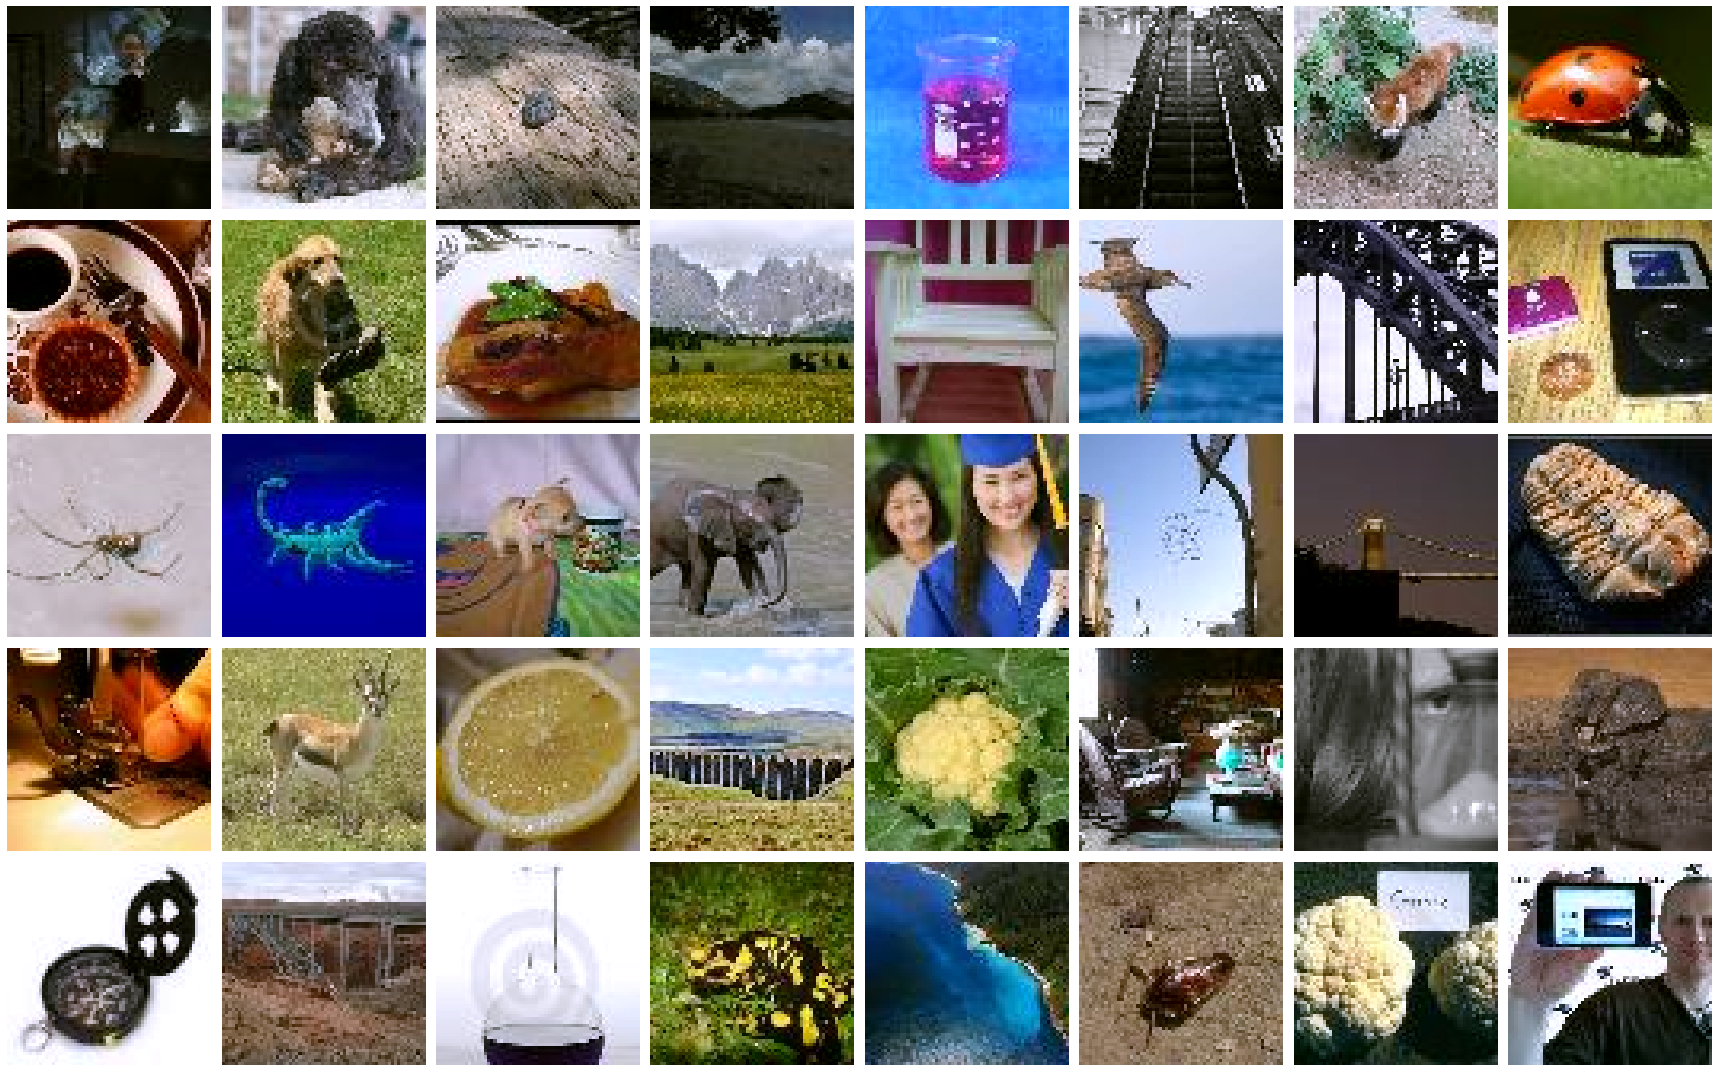
\includegraphics[width=0.9\textwidth]{./images/tinyimagenet.png}
	\caption{Tiny Imagenet}
\end{figure}

\newpage

\subsubsection{Internal and External Parts of Cars}
The \textit{Internal and External Parts of Cars} dataset \cite{internalexternal} is a subset of the CompCars \cite{carparts} dataset.
It contains images of different internal and external car parts.
In total there are 27.618 images from 8 different classes.
The dataset is used in the experiments to test zero-shot classification performance and a subset of 20 images per class is used to measure the performance on very small datasets.

\begin{figure}[h]
    \centering
    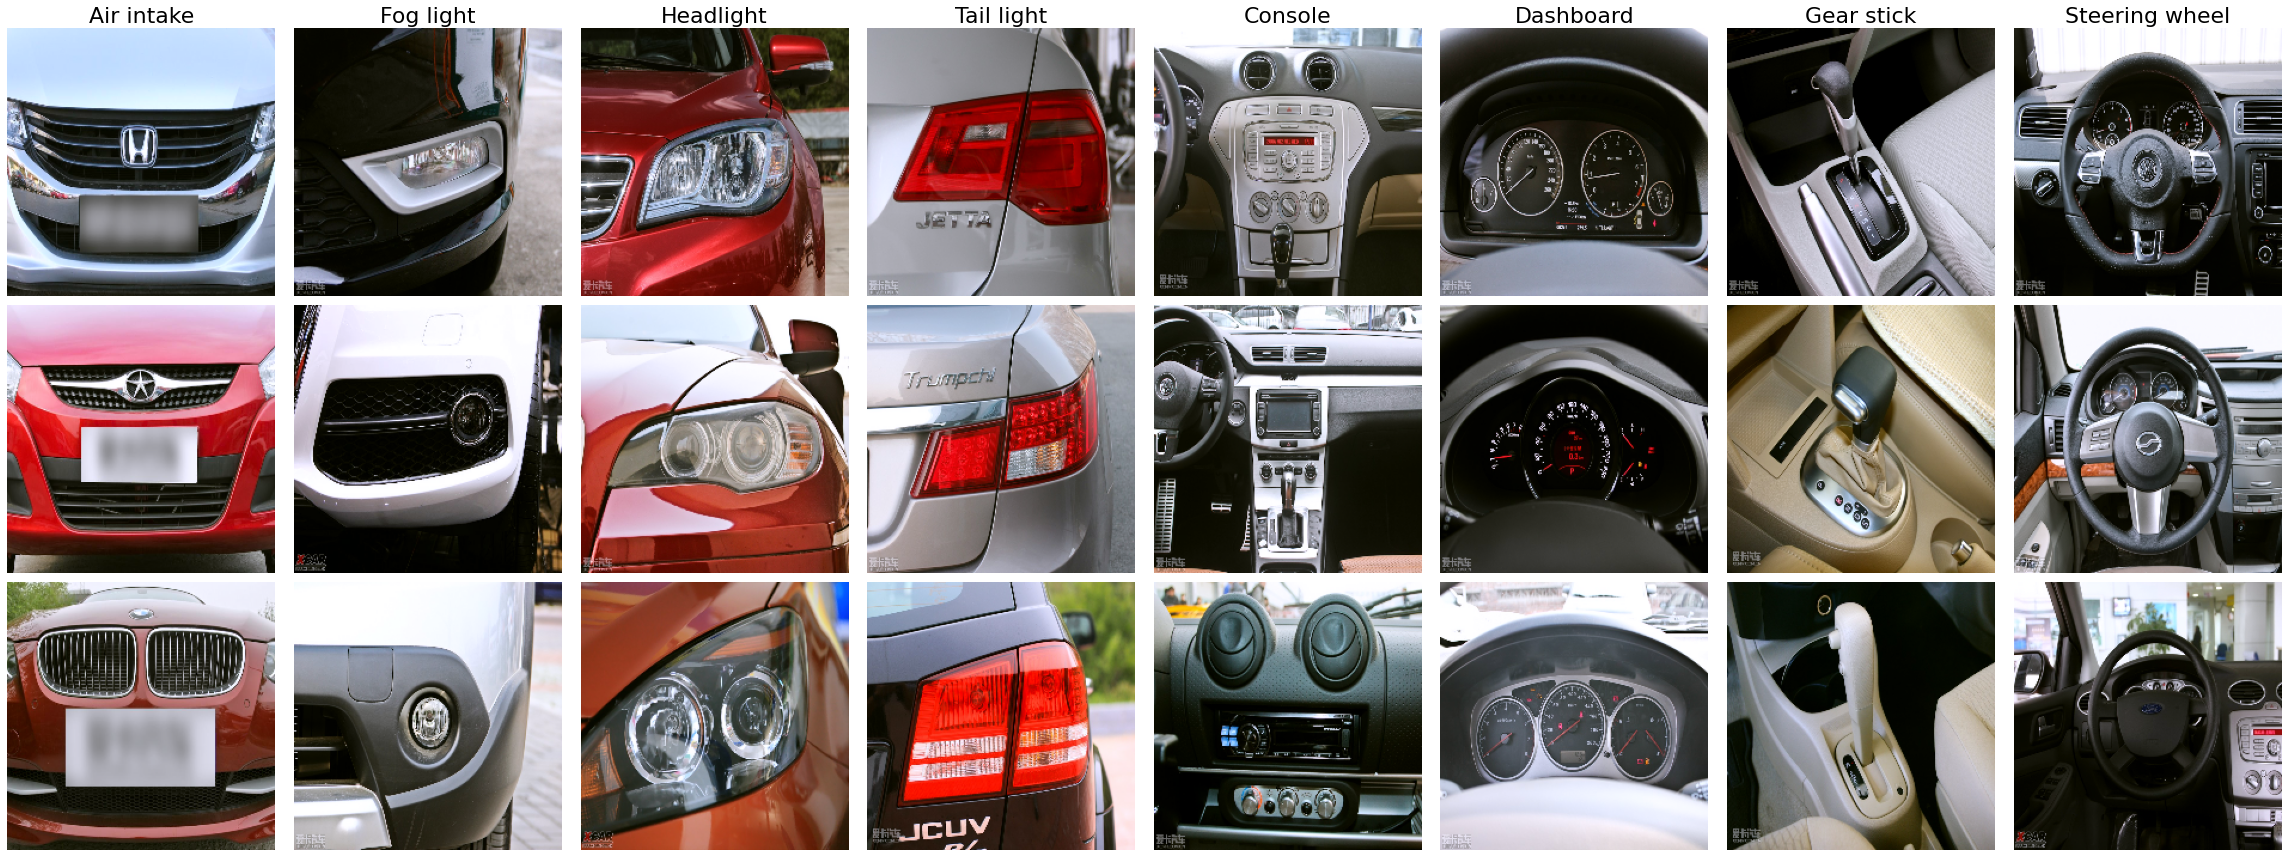
\includegraphics[width=\textwidth]{./images/carparst.png}
	\caption{Internal and External Parts of Cars}
\end{figure}


\newpage


\chapter{Methods}
\section{Siamese networks}
A Siamese neural network is a neural network that consists of two or more identical networks.\cite{signatureVerification}
To generate deep image embeddings from images, these multiple networks are only used in the training step,
where the embeddings are calculated for each image and a loss function is used to minimize or maximize the distance between the embeddings,
depending on the task. For later inference only on of the networks is used.

\begin{figure}[h]
    \centering
    \subfloat[\centering Positives]{{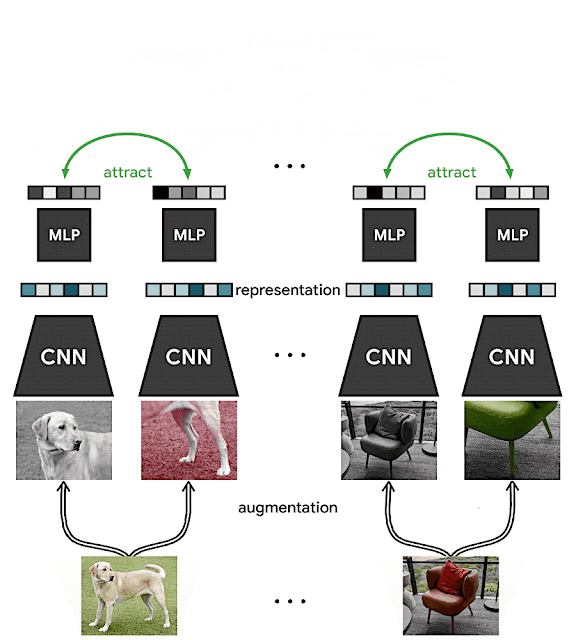
\includegraphics[width=5cm]{./images/siamese_attract.png} }}
    \qquad
    \subfloat[\centering Negatives]{{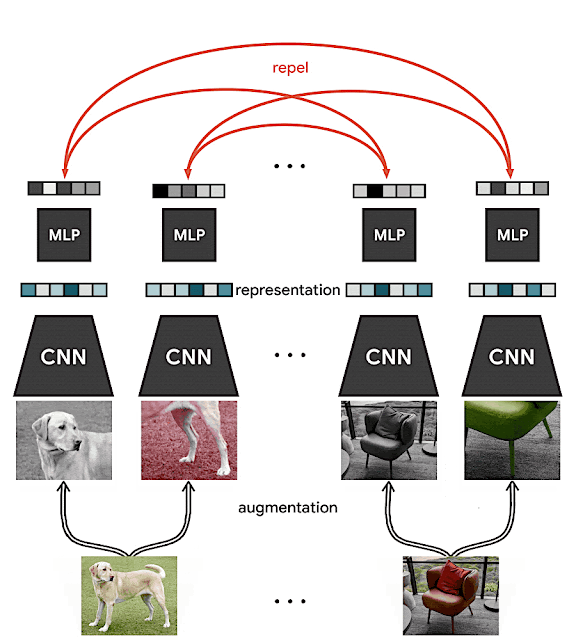
\includegraphics[width=5cm]{./images/siamese_repel.png} }}
    \caption{Similarity Training in Siamese Networks \cite{simclrartikle}}
\end{figure}

Frameworks like SimCLR\cite{simclr} don't use multiple networks for training, but instead use a single network that processes every image in a mini batch.
The resulting embeddings are then sorted by labels and grouped into positives and negatives.
Then a loss function is used to minimize distance between the positives and maximize the distance between the negatives.
This approach is a lot faster and uses less memory than using multiple networks.
\\
There is also the \textit{PyTorch Metric Learning}\cite{musgrave2020pytorch} library available for this task, that implements the same approach for generic pytorch models.

\section{Backbones}
The following Backbones were used to perform the feature extraction:
\begin{itemize}
	\item ResNet 50 \cite{resnet}
 	\item EfficientNetV2 \cite{EfficientNetV2}
  	\item MobilNetV3 \cite{MobilNetV3}
    \item DenseNet \cite{DenseNet}
    \item Vit \cite{ViT}
    \item Swin \cite{liu2021swin}
\end{itemize}

\section{Losses}
The following contrastive loss functions were used to optimize the embedding vectors:
\begin{itemize}
	\item ContrastiveLoss \cite{ContrastiveLoss}
 	\item TripletLoss \cite{TripletLoss}
  	\item SupConLoss \cite{SupConLoss}
    \item SNRLoss \cite{SNRLoss}
    \item NTXentLoss \cite{simclr}
\end{itemize}

\newpage

\section{Augmentation techniques}
The following augmentation techniques were used to augment the training data:
\begin{itemize}
	\item AutoAugment \cite{AutoAugment}
 	\item RandAugment \cite{RandAugment}
  	\item TrivialAugmentWide \cite{TrivialAugmentWide}
\end{itemize}

\section{t-SNE}
T-distributed stochastic neighbor embedding (t-SNE) is a statistic method for embedding visualization.
It is a technique for dimensionality reduction that is particularly well suited for the visualization of high-dimensional data.
The algorithm is based on the idea of finding a low-dimensional representation of the data that preserves the local structure of the data.

\begin{figure}[h]
    \centering
    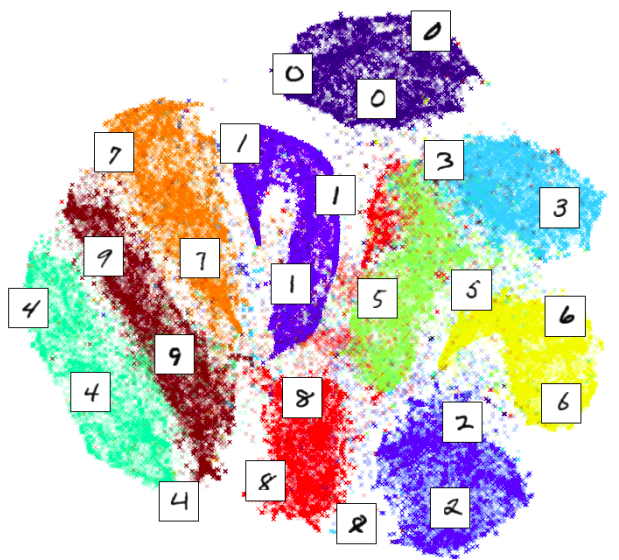
\includegraphics[width=0.5\textwidth]{./images/tsne-mnist.png}
	\caption{t-SNE visualization of MNIST}
\end{figure}

\newpage
\chapter{Results and Discussion}

\newpage

\section{Backbone performance}
In this experiment different backbones were used to train a siamese network for five epochs on a subset of 50 classes of the Tiny ImageNet dataset.
No augmentations were used.
Each network had a target embedding size of 256, used the TripletLoss metric and was initialized with pretrained ImageNet weights.

\subsubsection*{Results}
\begin{wraptable}{r}{5cm}
	\begin{tabular}{ | c | c | }
		\hline
		Backbone & F1-Score \\ 
		\hline
		ResNet50 & 0.664 \\ 
		\hline
		EfficientNetV2 L & 0.540 \\ 
		\hline
		MobilNetV3 & 0.367 \\ 
		\hline
		DenseNet169 & 0.612 \\ 
		\hline
		ViT & 0.893 \\ 
		\hline
		Swin & 0.934 \\ 
		\hline
	\end{tabular}
\end{wraptable} 
Although ViT and Swin are a lot slower and need more memory than the other backbones they perform a lot better.
This property can also be observed in NLP tasks, where transformers originated from.
Small models like MobilNetV3 and EfficientNet seem to struggle to generate good embeddings for all classes.
They would probably perform a lot better if the embedding tasks contains less classes.
The ResNet50 baseline generates good embeddings and even outperforms the larger DenseNet169 backbone.

\vspace{0.5cm}

\begin{figure}[h]
	\centering
	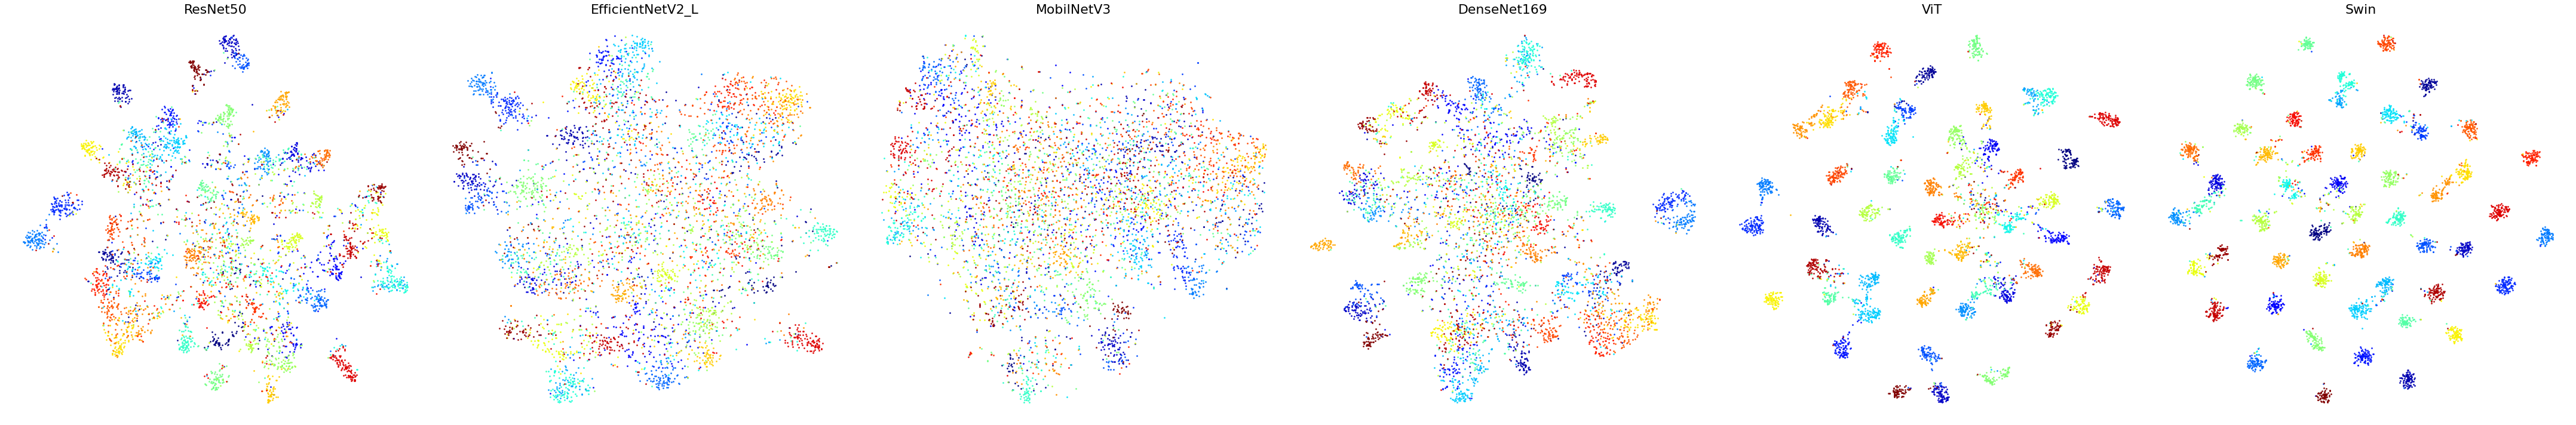
\includegraphics[width=0.9\textwidth]{../plots/backbones.png}
	\caption{t-SNE visualization of backbones}
\end{figure}

\newpage

\section{Significance of Loss Functions}

In this experiment different loss functions were used to train a siamese network for five epochs on a subset of 50 classes of the Tiny ImageNet dataset.
No augmentations were used.
As a backbone ResNet50 was used.
The network had a target embedding size of 256 and was initialized with pretrained ImageNet weights.


\subsubsection*{Results}
\begin{wraptable}{r}{5cm}
	\begin{tabular}{ | c | c | }
		\hline
		Loss & F1-Score \\ 
		\hline
		ContrastiveLoss & 0.650 \\ 
		\hline
		TripletLoss & 0.660 \\ 
		\hline
		SupConLoss & 0.709 \\ 
		\hline
		SNRLoss & 0.685 \\ 
		\hline
		NTXentLoss & 0.618 \\ 
		\hline
	\end{tabular}
\end{wraptable} 

The SupConLoss function is the best performing loss function.
It is also the only loss function that expects the data to be labeled and is optimized for supervised learning.
The other loss functions are more general and can also be used for unsupervised learning.
We trained the network with labeled data, so its expected that the SupConLoss function performs better than the other loss functions.

\vspace{0.5cm}

\begin{figure}[h]
	\centering
	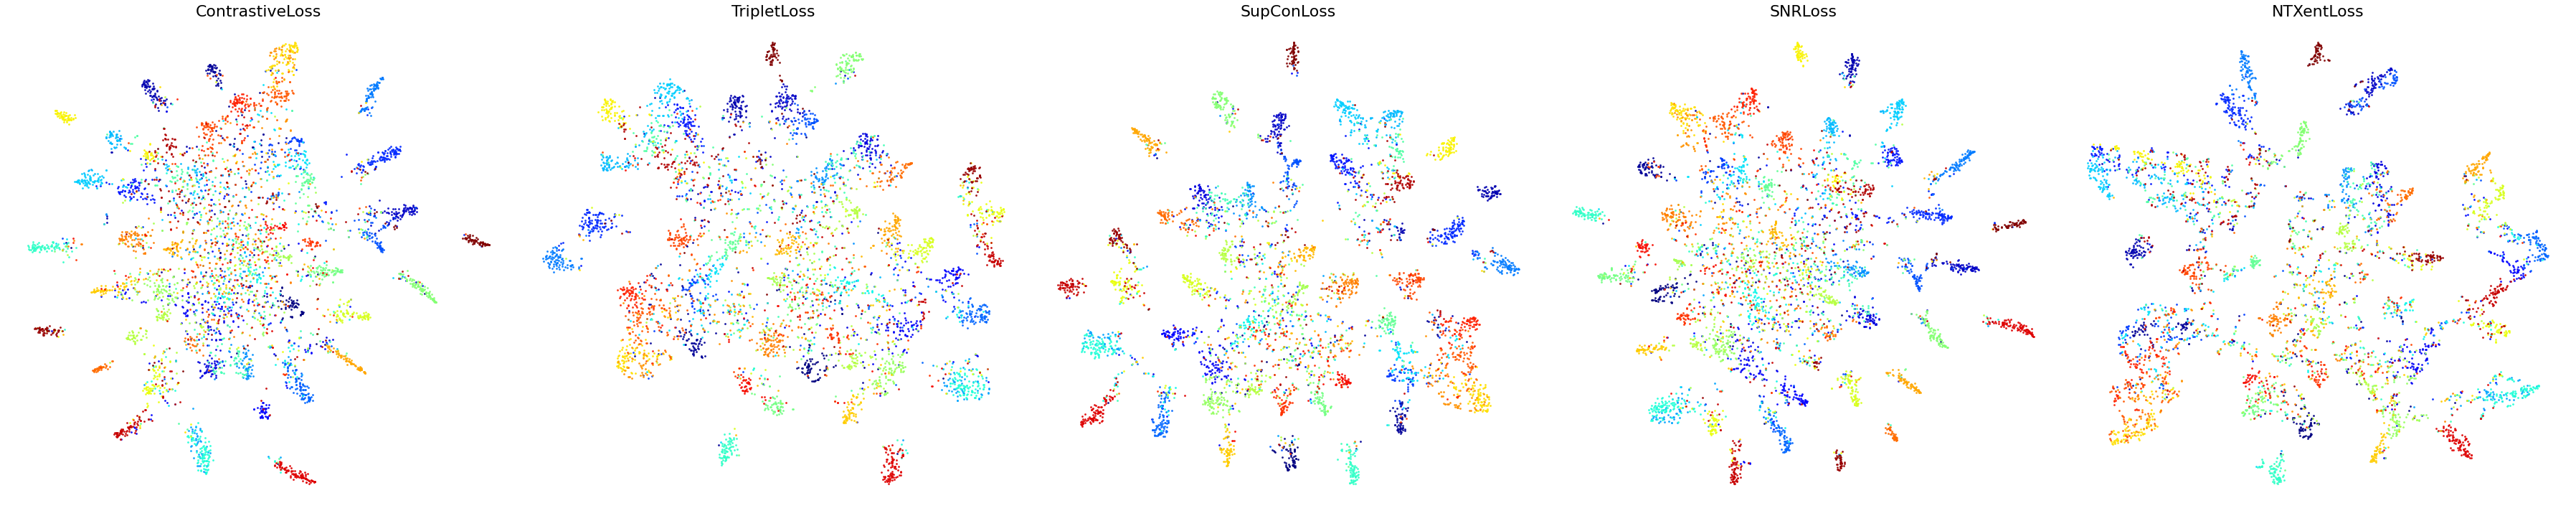
\includegraphics[width=0.9\textwidth]{../plots/losses.png}
	\caption{t-SNE visualization of loss functions}
\end{figure}

\newpage

\section{Differences in Embedding Sizes}

In this experiment different embedding sizes were used to train a siamese network for five epochs on a subset of 50 classes of the Tiny ImageNet dataset.
No augmentations were used.
As a backbone ResNet50 was used.
The network used the SupConLoss metric and was initialized with pretrained ImageNet weights.


\subsubsection*{Results}
\begin{wraptable}{r}{5cm}
	\begin{tabular}{ | c | c | }
		\hline
		Embedding Size &  F1-Score \\ 
		\hline
		64 &  0.654 \\ 
		\hline
		128 & 0.683 \\ 
		\hline
		256 & 0.712 \\ 
		\hline
		512 & 0.719 \\ 
		\hline
		1024 & 0.724  \\ 
		\hline
		2048 & 0.731 \\ 
		\hline
	\end{tabular}
\end{wraptable} 

The performance of the network get better with higher embedding sizes.
This effect seams to plateau at an embedding sizes of 1024.
With bigger embedding sizes the parameters of the model increase exponentially and we need a lot more calculations to perform KNN-Searches on the generated embeddings.
So its not possible to scale the embedding size indefinitely.

\vspace{0.5cm}

\begin{figure}[h]
	\centering
	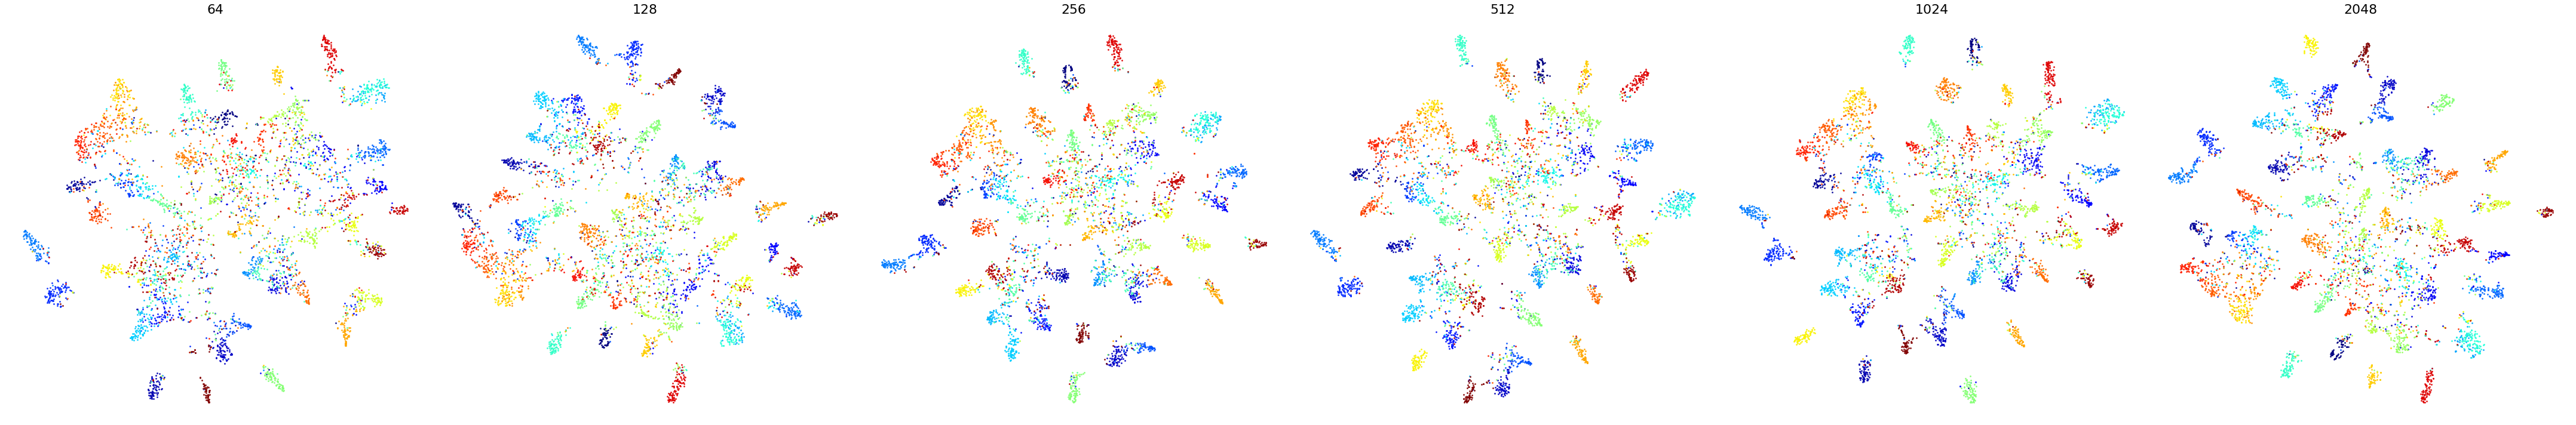
\includegraphics[width=0.9\textwidth]{../plots/embedding_size.png}
	\caption{t-SNE visualization of embedding sizes}
\end{figure}


\chapter{Conclusion}

\newpage

\bibliography{refs}

\end{document}